\documentclass[../PHYS306Notes.tex]{subfiles}

\begin{document}
\section{Lecture 28}
\subsection{Lecture Notes - Differential Cross Section}
\subsubsection{Review}
Cross section = area of ring of radius $b$ and width $db$. Particles hitting the ring between $b$ and $b + db$ are scattered by an angle between $\theta$ and $\theta + d\theta$. Scattered onto a larger ring on a sphere with scallering nucleus in center. The solid angle of the entire ring is:
\[d\Omega = \frac{2\pi R\sin\theta Rd\theta}{R^2} = 2\pi\sin\theta d\theta\]
And the solid angle of a small area is given by:
\[d\Omega = \frac{d\phi R\sin\theta Rd\theta}{R^2} = \sin\theta d\phi d\theta\]
This notion is useful as often our particle detectors cover a certain fraction of the area. 
\begin{center}
    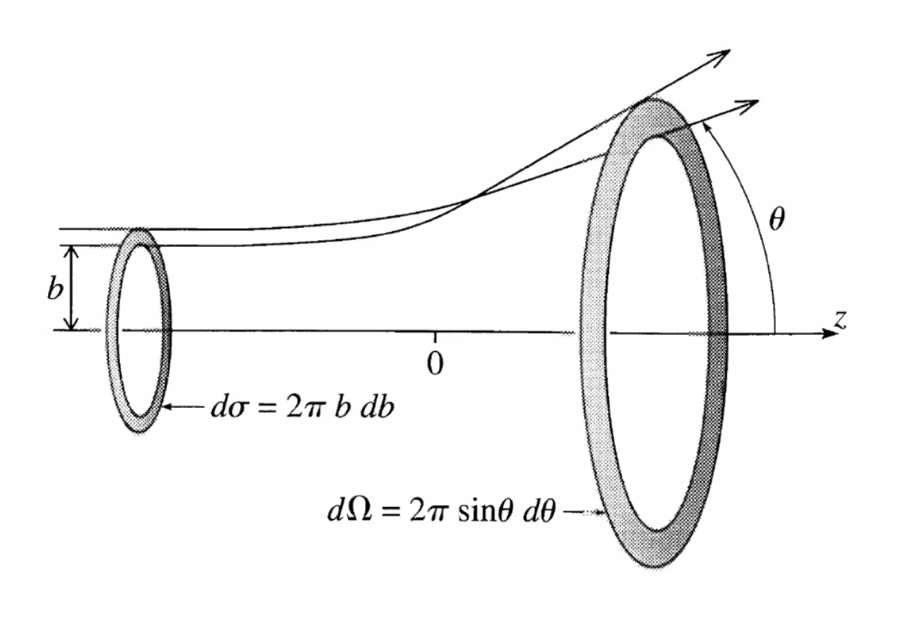
\includegraphics[scale=0.5]{Lecture-28/l28-img1.png}
\end{center}
The ratio between the $d\sigma$ of the first ring and the $d\Omega$ of the second ring is the the differential cross section, which is:
\[\dod{\sigma}{\Omega} = \frac{b}{\sin\theta}\abs{\dod{b}{\theta}}\]
Where $d\sigma = 2\pi b db$ and $d\Omega = 2\pi \sin\theta d\theta$. The task today is then to obtain $b$ in terms of $\theta$ ($b(\theta)$). Today, we will consider the case where our target is fixed (i.e. a heavy target) and try to describe the trajectory of this scenario. This is just the two body central force problem (as covered in PHYS 216), with the only difference that the orbits are open and not closed.

\subsubsection{Calculation of the differential cross-section - The Kepler Approach}
We first remark that this chapter is interesting as not only is it highly relevant to research fields (e.g. particle physics) but also puts something that we know (the two-body problem) into a new context. We now move onto solving this two-body central force problem. The total energy of the system in polar coordinates is given by:
\[E = \frac{m}{2}\left(\dot{r}^2 + r^2\dot{\phi}^2\right) + U(r) = \text{Const}\]
Where $U(r)$ is the scattering potential. Here the energy is conserved. Another quantity that is conserved is the angular momentum:
\[L = mr^2\dot{\phi} = \text{Const}\]
From this, we can immediately write:
\[r^2\dot{\phi}^2 = \frac{L^2}{m^2r^2}\]
Hence sustituting this into the energy expression to obtain everything in terms of $r$, we have:
\[E = \frac{m}{2}\left(\dot{r}^2 + \frac{L^2}{m^2r^2}\right) + U(r)\]
We can therefore solve for $\abs{\dot{r}}$:
\[\abs{\dot{r}} = \sqrt{\frac{2E}{m} - \frac{2U(r)}{m} - \frac{L^2}{m^2r^2}}\]
We have a two body problem, but it is effectively a one body problem. We may introduce an "effective potential":
\[U_{eff} = U(r) + \frac{L^2}{2mr^2}\]
Since we know that $\phi(t)$ is monotonic, we may write:
\[\abs{\dot{\phi}} = \frac{\abs{L}}{mr^2}\]
Dividing the $\dot{\phi}$ equation by the $\dot{r}$ equation, we get:
\[\frac{\abs{\dot{\phi}}}{\abs{\dot{r}}} = \abs{\dod{\phi}{r}} = \frac{\frac{\abs{L}}{mr^2}}{\sqrt{\frac{2E}{m} - \frac{2U(r)}{m} - \frac{L^2}{m^2r^2}}}\]
We can from this expression obtain the trajectory in the following way. The particle is incoming with impact parameter $b$, and deflects off by angle $\theta$. There is some closest point of approach $r_{min}$ that divides the trajectory into two pieces, that is, the trajectory is symmetric about $r_{min}$. Call the angle at this point $\Delta \phi/2$. This can be visualized as follows:
\begin{center}
    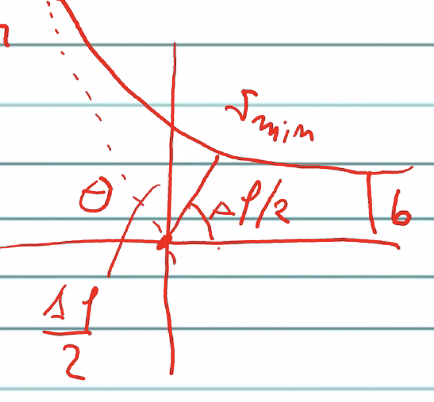
\includegraphics[scale=0.7]{Lecture-28/l28-img2.png}
\end{center}
We therefore have that:
\[\Delta \phi(r) = 2\int_{r_{min}}^\infty \frac{\frac{L}{r^2}}{\sqrt{2m(E-U) - \frac{L^2}{r^2}}}\]
Note that we obtain $r_{min}$ by solving for the turnaround point, i.e the energy equals the effective potential (the kinetic energy is zero) so:
\[2m(E - U) = \frac{L^2}{r_{min}^2}\]
However, all of our equations are in terms of $L$ and $E$;  should recast these in terms of physical parameters. Set:
\[E = T_{\infty} = \frac{m}{2}v_{\infty}^2\]
and 
\[L = \abs{\v{r} \times \v{p}_{\infty}} = mbv_{\infty}\]
Hence we may write:
\[\Delta \phi = 2b\int_{r_{min}}^\infty \frac{dr}{r^2\sqrt{1 - \frac{2U(r)}{mv_{\infty}^2} - \frac{b^2}{r^2}}}\]
So we have expressed the integral purely in terms of the mass, velocity, and impact parameter, which are all measureable variables. Note that this solution isn't really scattering; this is a very general solution to the two-body problem. 
We can now apply it to some relevant scattering scenarios to obtain the differential cross section.

\subsubsection{Example - Hard Sphere Differential Cross-Section}
In this case, $r_{min} = R$ (closest point of approach is just the surface of the sphere), and $V(r) = 0$ for $r > R$ (the particles don't see each other). For this case, we have:
\[\Delta \phi = 2b\int_R^\infty\frac{dr}{r^2\sqrt{1 - \frac{b^2}{r^2}}}\]
The middle term is zero as the potential is zero in the region of interest. This integral is solvable analytically, but we may very well just look this up instead of undergoing a tedious calculation:
\[\Delta \phi = 2\arcsin(\frac{b}{R})\]
Rearranging, we get:
\[b = R\sin(\frac{\Delta \phi}{2})\]
According to the picture we have drawn, $\Delta \phi + \theta = \pi$, so we can convert this to be in terms of $\theta$, which works out to be:
\[b = R\cos(\frac{\theta}{2}) = b(\theta)\]
Now, all is left to do is to calculate the differential cross section:
\[\dod{\sigma}{\Omega} = \frac{b}{\sin\theta}\abs{\dod{b}{\theta}} = \frac{R\cos(\frac{\theta}{2})}{\sin\theta}\abs{-\frac{R}{2}\sin(\frac{\theta}{2})} = \frac{R^2}{2\sin\theta}\cos(\frac{\theta}{2})\sin(\frac{\theta}{2}) = \frac{R^2}{2\sin\theta}\frac{1}{2}\sin(\theta) = \frac{R^2}{4}\]
Hence calculating $\sigma_{tot}$ (total cross section) we have:
\[\sigma_{tot} = \int \dod{\sigma}{\Omega}d\Omega = \int \frac{R^2}{4}d\Omega = \pi R^2\]
Which is a good sanity check, as it agrees with what we found on Monday!

\subsubsection{Example - Coloumb Potential Differential Cross-Section}
In this case, we have that:
\[U = -\frac{\beta}{r}\]
Where $\beta = -kqQ < 0$ (repulsive). The procedure is exactly the same, but the integral is just harder. 
\[\Delta \phi = 2b\int_{r_{min}}^\infty \frac{dr}{r\sqrt{r^2 + \frac{2\beta r}{mv_{\infty}} - b^2}}\]
\[\Delta \phi = \left.2\arccos(\frac{1 - \frac{mv_\infty^2 b^2}{\beta}}{\sqrt{1 + \left(\frac{mv_{\infty}^2b}{\beta}\right)^2}})\right|_{r_{min}}^{\infty}\]
Evaluating at the bounds, we get:
\[\Delta \phi = 2\arccos(\frac{1}{\sqrt{1 + \left(\frac{mv_\infty b}{\beta}\right)^2}})\]
(this is the term at infinity, the term at $r_{min}$ vanishes, as the value is $2\arccos(-1) = 2\pi$ and $\phi = \phi + 2\pi$). Hence solving for $b(\theta)$ we have:
\[b(\theta) = \frac{1}{mv_{\infty}^2}\sqrt{\frac{1}{\sin^2(\frac{\theta}{2})} - 1}\]
Using this, we find the differential cross section:
\[\frac{d\sigma}{d\Omega} = \frac{k^2q_1^2q_2^2}{16E^2}\frac{1}{\sin^4(\frac{\theta}{2})}\]
Plotting the Rutherford cross section, we find:

Where we have a characteristic divergence at the origin and a rapid decrease, with a value of $1$ at $\pi$. 
\begin{center}
    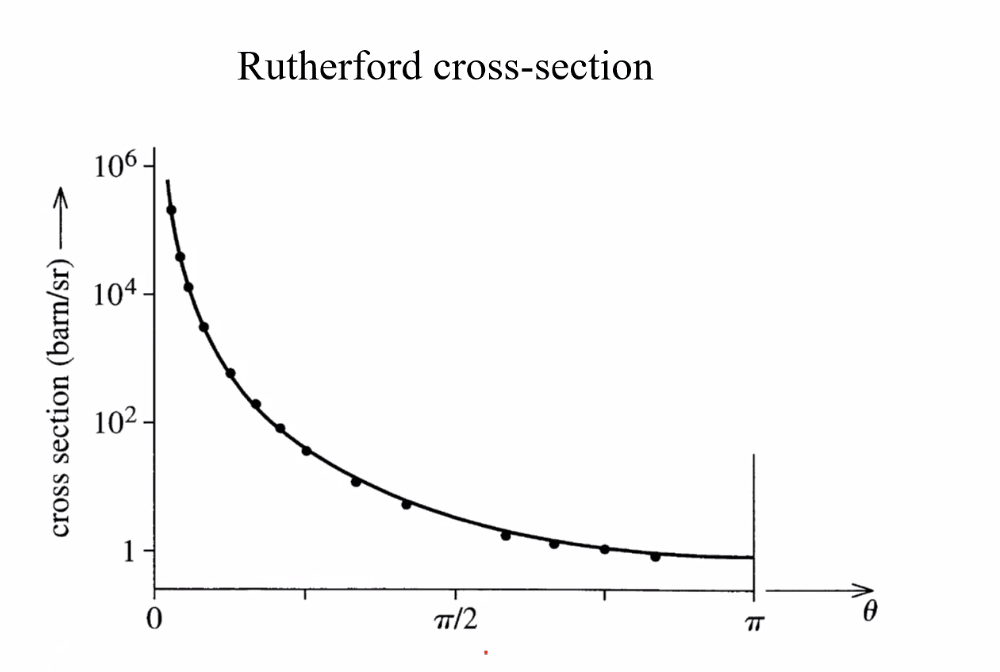
\includegraphics[scale=0.5]{Lecture-28/l28-img3.png}
\end{center}
Question: What is the total cross section?
\begin{s}
$\sigma = \int\dod{\sigma}{\Omega}d\Omega = \infty$ due to the divergence at the origin. This can be traced back to the $\frac{1}{r}$ type behavior of the Columb potential. 
\end{s}
A remark: One could state that this (classical treatment) is nonsense and we require a quantum treatment. Luckily, the classical treatment actually does work out in this case (due to the Coulomb potential in particular) but for a full description we require a quantum formulation, which is something we can expect to see in Graduate school QM. Next day we will look at the center of mass lab frame, and how we treat scattering off of nuclei that are not infinitely heavy. 
\end{document}